%TODO: ARREGLAR EJERCICIO 1B
\documentclass{article}
\usepackage[utf8]{inputenc}
\usepackage[spanish]{babel}
\usepackage{graphicx, graphics, float, hyperref}
\usepackage{listings}
\usepackage[a4paper, total={6in, 10in}]{geometry}

\title{SSO Práctica 1 Sesión 2}
\author{Andrés Merlo Trujillo}
\date{}
\hypersetup{
    colorlinks=true,
    linkcolor=black,
}

\begin{document}

\maketitle

\tableofcontents

\newpage
%\addcontentsline{toc}{section}{Ejercicio 1}
%\section*{Ejercicio 1}
%\begin{figure}[H]
%    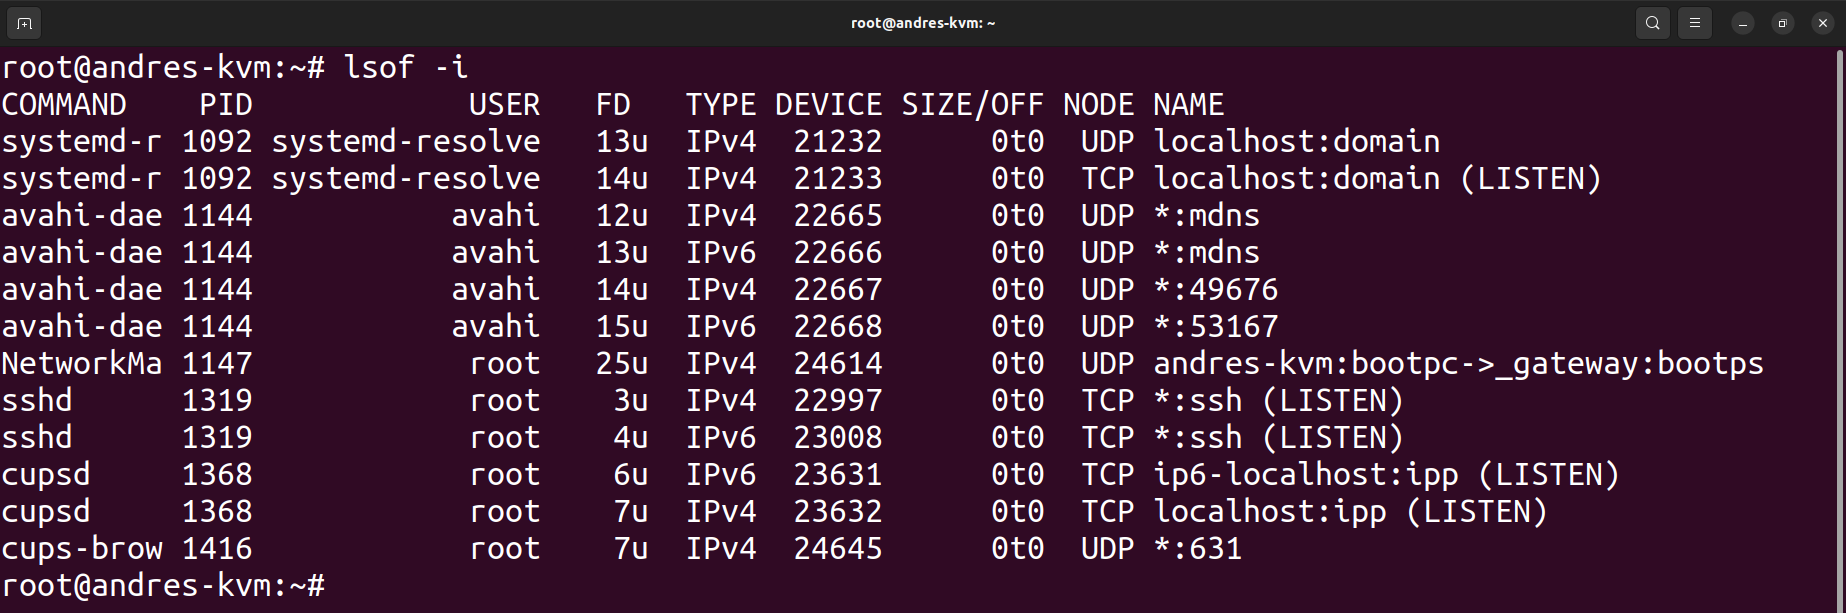
\includegraphics[width=\textwidth]{imagenes/lsofi.png}
%\end{figure}

\addcontentsline{toc}{section}{Ejercicio 1}
\section*{Ejercicio 1}
Con la orden \verb|aa-status| o la orden \verb|apparmor_status| se pueden ver los perfiles activos en Ubuntu:

%foto de los perfiles
%caption: como se puede ver hay 42 perfiles cargados.

Ahora voy a elegir el perfil \verb|/usr/bin/freshclam|, para poder ver el archivo del perfil asociado basta con irse al directorio \verb|/etc/apparmor.d| y el archivo se denomina igual que la ruta absoluta del mismo, pero en vez de usar ``/'' se utilizan puntos. Por tanto, el archivo deseado es: \verb|/etc/apparmor.d/usr.bin.freshclam|.

%foto del archivo

%otra foto

Las compoenntes principales son las siguientes:

%https://manpages.debian.org/jessie/apparmor/apparmor.d.5.en.html

\begin{itemize}
    \item \verb|#include <tunables/global>| Carga un archivo que contiene las definiciones de las variables.
    \item \verb|/usr/bin/freshclam| Ruta absoluta del binario.
    \item \verb|#include <abstractions/base>| Obtiene los componentes de los perfiles de AppArmor para simplifcar el desarrollo de perfiles.
    \item \verb|#include <abstractions/nameservice>| Incluye las reglas para permitri DNS, LDAP, NIS, SMB, contraseñas de usuarios y grupos, serivicos y ``lookups'' de protocolos
    \item \verb|#include <abstractions/user-tmp>| Permite acceder a los directorios temporales
    \item \verb|#include <abstractions/openssl>| Permite acceder a los archivos correspondientes a OpenSSL.
    \item \verb|{,var/}| Permite eliminar lineas innecesarias, poniendo los directorios similares dentro de la lista entre lalves. En este caso las opciones son \verb|/run/clamav/freshclam.pid| y \verb|/var/run/clamav/freshclam.pid|
    %\item \verb|... -> &man_groff| Utiliza el perfil referenciado en la derecha cuando \verb|man| utiliza algun comando de la izquierda.
    %\item \verb|profile ... {| Perfiles secundarios que se ejecutarán cuando estos sean llamados desde el principal. Por ejemplo, mediante el enlace de otro comando desde el perfil principal cuando \verb|freshclam| lo llame.
    %\item \verb|#include <abstractions/console>| Incluye acceso de lectura y escritura a los archivos de dispositivo que controlan las terminales virtuales, sshd, xterm, etc. Es necesario para proogramas que interaccionan con el usuario.
    \item \verb|capability ...| Indica las capabilities que tiene permitidas hacer en el sistema. El listado de todas ellas se puede ver usando \verb|man 7 capabilites|.
    \item \verb|owner archivo| Indica que solo puede accder al archivo indicado si es el propietario del mismo.
    \item \verb|deny archivo| Deniega el acceso al archivo indicado.
\end{itemize}

Además, aparecen variables del tipo ``@{\dots}'', el valor de estas variables se almacenan en \verb|/etc/apparmor.d/file| donde file es el nombre de la variable. Las que aparecen en este perfil son:

%foto de proc

\begin{itemize}
    \item \textbf{@\{HOME\}: }Lista de todos los \verb|home| de los usuarios, incluido el root.
    \item \textbf{@\{PROC\}: }Directorio donde procfs es montado.
\end{itemize}

Se puede ver que contiene una lista de archivos y directorios junto con sus permisos, estos son los archivos o directorios a los que puede tener acceso, determinado por los switches que se muestran a continuacion:

\begin{itemize}
    \item \textbf{r: }Modo lectura
    \item \textbf{w: }Modo escritura
    \item \textbf{a: }Modo adjuntar (append)
    \item \textbf{k: }Modo de bloqueo de archivo
    \item \textbf{l: }Modo de enlace
    \item \textbf{ux: }Modo de ejeccion sin restricciones
    \item \textbf{Ux: }Modo de ejeccion sin restricciones. Ademas, limpia el entorno (scrub the environment)
    \item \textbf{px: }Ejecucion discreta del perfil
    \item \textbf{Px: }MOdo de ejecucion discreta del perfil. Ademas, limpia el entorno (scrub the environment)
    \item \textbf{ix: }MOdo de ejecucion heredada
    \item \textbf{m: }Permite \verb|PROT_EXEC| con llamadas a \verb|mmap|
    \item \textbf{Cx: }Permite transiciones a un perfil hijo. Con la C mayuscula se usa ``secure exec'' de glibc.
\end{itemize}


\addcontentsline{toc}{section}{Ejercicio 2}
\section*{Ejercicio 2}
Voy a generar un perfil para el programa \verb|nano|, para saber su ruta absoluta se puede usar la orden \verb|which nano|:

%foto de which nano

Ahora para generar el perfil se ejecuta el comando \verb|aa-genprof /usr/bin/nano|:

%fotos

Ahora pide que abramos el programa a perfilar y pulsemos en el boton de escanear.

Es recomendable abrir el manual de capabilites para ver que significa cada capability con \verb|man 7 capabilities|.

%foto de dar_read_search

Esto permite saltarse las comoprobaciones de permisos de lecutra sobre el archivo y las comprobaciones sobre el directorio de permiso de lectura y ejecucion. Es mejor denegarlo con la tecla ``D''.

%foto nanorc
nanorc es un archivo con las configuraciones personlaizadas para el editor, al ser un archivo inofensivo se puede permitir su uso.



\end{document}

%\begin{figure}[H]
%    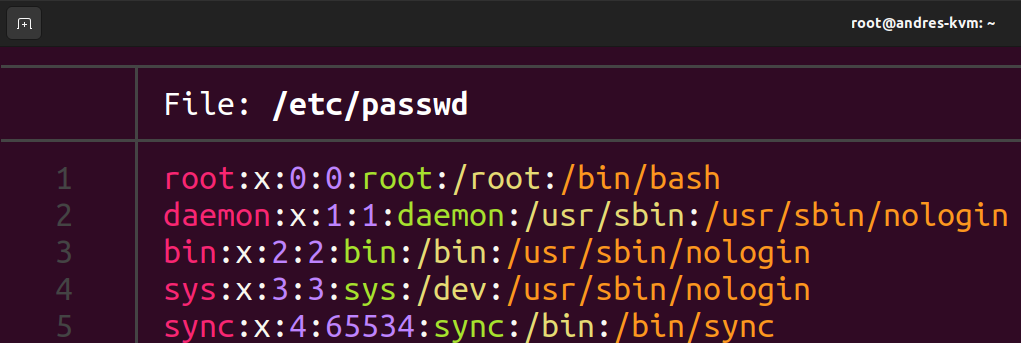
\includegraphics[width=\textwidth]{imagenes/passwdfile.png}
%    \caption{Ejemplo de entradas en el archivo.}
%\end{figure}